\documentclass[border=10pt]{standalone}
\usepackage{tikz}
\usetikzlibrary{arrows,positioning,shapes.geometric}
\begin{document}
\


\tikzset{every picture/.style={line width=0.75pt}} %set default line width to 0.75pt        

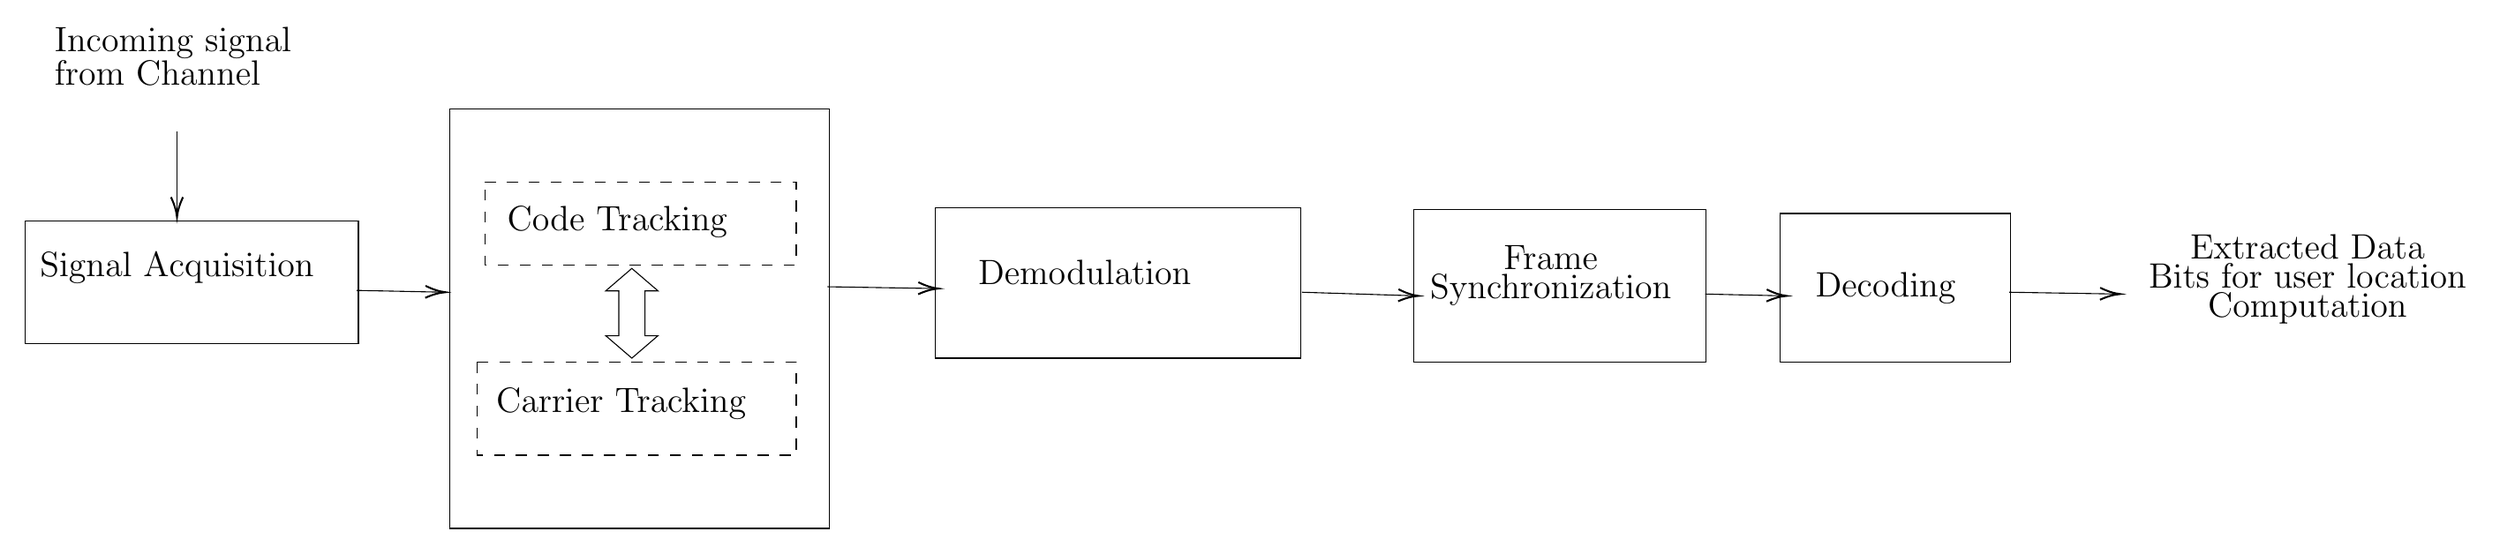
\begin{tikzpicture}[x=0.75pt,y=0.75pt,yscale=-1,xscale=1]
%uncomment if require: \path (0,421); %set diagram left start at 0, and has height of 421

%Shape: Rectangle [id:dp3971746291758471] 
\draw  [dash pattern={on 4.5pt off 4.5pt}] (262,160) -- (432,160) -- (432,205) -- (262,205) -- cycle ;
%Shape: Rectangle [id:dp25845085129393275] 
\draw   (11,181) -- (193,181) -- (193,248) -- (11,248) -- cycle ;
%Shape: Rectangle [id:dp4338649750832799] 
\draw  [dash pattern={on 4.5pt off 4.5pt}] (258,258) -- (432,258) -- (432,309) -- (258,309) -- cycle ;
%Straight Lines [id:da025296917723176437] 
\draw    (94,132) -- (94,177) ;
\draw [shift={(94,179)}, rotate = 270] [color={rgb, 255:red, 0; green, 0; blue, 0 }  ][line width=0.75]    (10.93,-3.29) .. controls (6.95,-1.4) and (3.31,-0.3) .. (0,0) .. controls (3.31,0.3) and (6.95,1.4) .. (10.93,3.29)   ;
%Shape: Rectangle [id:dp16992156871850217] 
\draw   (243,120) -- (450,120) -- (450,349) -- (243,349) -- cycle ;
%Straight Lines [id:da034679195397693485] 
\draw    (192,219) -- (238.5,219.96) ;
\draw [shift={(240.5,220)}, rotate = 181.18] [color={rgb, 255:red, 0; green, 0; blue, 0 }  ][line width=0.75]    (10.93,-3.29) .. controls (6.95,-1.4) and (3.31,-0.3) .. (0,0) .. controls (3.31,0.3) and (6.95,1.4) .. (10.93,3.29)   ;
%Up Down Arrow [id:dp0963447637089958] 
\draw   (328,219.25) -- (342.25,207) -- (356.5,219.25) -- (349.38,219.25) -- (349.38,243.75) -- (356.5,243.75) -- (342.25,256) -- (328,243.75) -- (335.13,243.75) -- (335.13,219.25) -- cycle ;
%Straight Lines [id:da4490352243030665] 
\draw    (449,217) -- (507.5,217.97) ;
\draw [shift={(509.5,218)}, rotate = 180.95] [color={rgb, 255:red, 0; green, 0; blue, 0 }  ][line width=0.75]    (10.93,-3.29) .. controls (6.95,-1.4) and (3.31,-0.3) .. (0,0) .. controls (3.31,0.3) and (6.95,1.4) .. (10.93,3.29)   ;
%Shape: Rectangle [id:dp8453662584022844] 
\draw   (508,174) -- (707.5,174) -- (707.5,256) -- (508,256) -- cycle ;
%Straight Lines [id:da8952050873529491] 
\draw    (708,220) -- (769.5,221.94) ;
\draw [shift={(771.5,222)}, rotate = 181.8] [color={rgb, 255:red, 0; green, 0; blue, 0 }  ][line width=0.75]    (10.93,-3.29) .. controls (6.95,-1.4) and (3.31,-0.3) .. (0,0) .. controls (3.31,0.3) and (6.95,1.4) .. (10.93,3.29)   ;
%Shape: Rectangle [id:dp25594644752156004] 
\draw   (769,175) -- (928.5,175) -- (928.5,258) -- (769,258) -- cycle ;
%Shape: Rectangle [id:dp8421655608501161] 
\draw   (969,177) -- (1094.5,177) -- (1094.5,258) -- (969,258) -- cycle ;
%Straight Lines [id:da35720729664785655] 
\draw    (928,221) -- (970.5,221.96) ;
\draw [shift={(972.5,222)}, rotate = 181.29] [color={rgb, 255:red, 0; green, 0; blue, 0 }  ][line width=0.75]    (10.93,-3.29) .. controls (6.95,-1.4) and (3.31,-0.3) .. (0,0) .. controls (3.31,0.3) and (6.95,1.4) .. (10.93,3.29)   ;
%Straight Lines [id:da16424451208563873] 
\draw    (1094,220) -- (1152.5,220.97) ;
\draw [shift={(1154.5,221)}, rotate = 180.95] [color={rgb, 255:red, 0; green, 0; blue, 0 }  ][line width=0.75]    (10.93,-3.29) .. controls (6.95,-1.4) and (3.31,-0.3) .. (0,0) .. controls (3.31,0.3) and (6.95,1.4) .. (10.93,3.29)   ;

% Text Node
\draw (18,197) node [anchor=north west][inner sep=0.75pt]   [align=left] {{\Large Signal Acquisition}};
% Text Node
\draw (273,172) node [anchor=north west][inner sep=0.75pt]   [align=left] {{\Large Code Tracking}};
% Text Node
\draw (267,271) node [anchor=north west][inner sep=0.75pt]   [align=left] {{\Large Carrier Tracking}};
% Text Node
\draw (771,193) node [anchor=north west][inner sep=0.75pt]   [align=left] {\begin{minipage}[lt]{107.24pt}\setlength\topsep{0pt}
\begin{center}
{\Large Frame }\\{\Large Synchronization}
\end{center}

\end{minipage}};
% Text Node
\draw (530,201) node [anchor=north west][inner sep=0.75pt]   [align=left] {{\Large Demodulation} };
% Text Node
\draw (987,208) node [anchor=north west][inner sep=0.75pt]   [align=left] {{\Large Decoding}};
% Text Node
\draw (1165,187) node [anchor=north west][inner sep=0.75pt]   [align=left] {\begin{minipage}[lt]{135.78pt}\setlength\topsep{0pt}
\begin{center}
{\Large Extracted Data }\\{\Large Bits for user location}\\{\Large Computation }
\end{center}

\end{minipage}};
% Text Node
\draw (26,74) node [anchor=north west][inner sep=0.75pt]   [align=left] {{\Large Incoming signal }\\{\Large from Channel}};


\end{tikzpicture}


   
\end{document}


